 \documentclass [12pt]{article} 

\usepackage {amsmath}
\usepackage {amsthm}
\usepackage {amssymb}
\usepackage {graphicx} 
\usepackage {float}
\usepackage {multirow}
\usepackage {xcolor}
\usepackage [ruled,vlined,commentsnumbered,titlenotnumbered]{algorithm2e} \usepackage {array} 
\usepackage {booktabs} 
\usepackage {url} 
\usepackage {parskip} 
\usepackage [margin=1in]{geometry} 
\usepackage [T1]{fontenc} 
\usepackage {cmbright} 
\usepackage [many]{tcolorbox} 
\usepackage [colorlinks = true,
            linkcolor = blue,
            urlcolor  = blue,
            citecolor = blue,
            anchorcolor = blue]{hyperref} 
\usepackage {enumitem} 
\usepackage {xparse} 
\usepackage {verbatim}
\usepackage{algpseudocode}
\usepackage{listings}
\usepackage{xcolor}
\lstset { %
    language=C++,
    backgroundcolor=\color{black!5}, % set backgroundcolor
    basicstyle=\footnotesize,% basic font setting
}
\newtheorem{theorem}{Theorem}
\newtheorem{remark}{Remark}
\newtheorem{lemma}[theorem]{Lemma}
\theoremstyle{definition}
\newtheorem{definition}{Definition}[section]
\newtheorem{claim}{Claim}






\DeclareTColorBox {Solution}{}{breakable, title={Solution}} \DeclareTColorBox {Solution*}{}{breakable, title={Solution (provided)}} \DeclareTColorBox {Instruction}{}{boxrule=0pt, boxsep=0pt, left=0.5em, right=0.5em, top=0.5em, bottom=0.5em, arc=0pt, toprule=1pt, bottomrule=1pt} \DeclareDocumentCommand {\Expecting }{+m}{\textbf {[We are expecting:} #1\textbf {]}} \DeclareDocumentCommand {\Points }{m}{\textbf {(#1 pt.)}} 

\begin {document} 

\vspace {1em} 
\begin {Instruction} 
Adapted From Virginia Williams' lecture notes.
\end {Instruction}  

{\LARGE \textbf {COMP 285 (NC A\&T, Spr `22)}\hfill \textbf {Lecture 27} } 

\begin{centering}
\section*{Dynamic Programmig V - 0/1 Knapsack and Maximal Independent Set}
\end{centering}

\section{The Knapsack Problem}
 
This is a classic problem, defined as the following:

We have $n$ items, each with a value and a positive weight. The $i$-th item has weight $w_i$ and value $v_i$. We have a knapsack that holds a maximum weight of $W$. Which items do we put in our knapsack to maximize the value of the items in our knapsack? For example, let’s say that $W = 10$; that is, the knapsack holds a weight of at most 10. Also suppose that we have four items, with weight and value:

\begin{table}[h!]
\centering
\begin{tabular}{c|c|c}
Item & Weight & Value \\
\hline
A & 6 &  25 \\
B & 3 & 13 \\
C & 4 & 15 \\
D & 2 & 8
\end{tabular}
\end{table}

We will talk about two variations of this problem, one where you have infinite copies of each item (commonly known as Unbounded Knapsack), and one where you have only one of each item (commonly known as 0-1 Knapsack). 

What are some useful subproblems? Perhaps it’s having knapsacks of smaller capacities, or maybe it’s having fewer items to choose from. In fact, both of these ideas for subproblems are useful. As we saw last lecture, the first idea is useful for the Unbounded Knapsack problem, and a combination of the two ideas is useful for the 0-1 Knapsack problem.

\subsection{The 0-1 Knapsack Problem}

We consider what happens when we can take at most one of each item. Going back to the initial example, we would pick item $A$ and item $C$, having a total weight of $10$ and a total value of $40$.

The subproblems that we need must keep track of the knapsack size as well as which items are allowed to be used in the knapsack. Because we need to keep track of more information in our state, we add another parameter to the recurrence (and therefore, another dimension to the DP table). Let $K(x, j)$ be the maximum value that we can get with a knapsack of capacity $x$ considering only items at indices from $1, \cdots , j$. Consider the optimal solution for $K(x, j)$. There are two cases: 

\begin{enumerate}
  \item Item $j$ is used in $K(x, j)$. Then, the remaining items that we choose to put in the knapsack must be the optimum solution for $K(x - w_j , j - 1)$. In this case, $K(x, j) = K(x - w_j , j - 1) + v_j$ .
  \item Item $j$ is not used in $K(x, j)$. Then, $K(x, j)$ is the optimum solution for K(x, j - 1). In this case, $K(x, j) = K(x, j - 1)$.
\end{enumerate}

So, our recurrence relation is: $K(x, j) = \max\{K(x -w_j , j -1) +v_j , K(x, j -1)\}$. Now, we’re done: we simply calculate each entry up to $K(W, n)$, which gives us our final answer. Note that this also runs in $O(nW)$ time despite the additional dimension in the DP table. This is because at each entry of the DP table, we do $O(1)$ work.

\begin{algorithm}
\caption{ZeroOneKnapsack(W, n, w, v)}
\label{alg:zerooneknapsack}
\begin{algorithmic}
\State \For{$j = 1, \cdots, n$}{
  $K[0,j] \gets 0$
}
\State \For{$x = 0, \cdots, W$}{
    $K[x, 0] \gets 0$
}
\State \For{$x = 1, \cdots, W$} {
  \State \For{$j = 1, \cdots, n$} {
    \State $K[x, j] \gets K[x, j-1]$
    \State \If {$w_j <= x$} {
        $K[x, j] = \max\{K[x - w_j, j-1] + v_j, K[x, j] \}$
    }
  }
}
\State \Return $K[W, n]$
\end{algorithmic}
\end{algorithm}


\section{The Independent Set Problem}

This problem is as follows: 

Say that we have an undirected graph $G = (V, E)$. We call a subset $S \subseteq V$ of vertices ``independent'' if there are no edges between vertices in $S$. Let vertex $i$ have weight $w_i$ , and denote $w(S)$ as the sum of weights of vertices in $S$. Given $G$, find an independent set of maximum weight $arg\max_{S\subseteq V} w(S)$.

Actually, this problem is NP-hard for a general graph $G$. However, if our graph is a tree, then we can solve this problem in linear time. In the following figure, the maximum weight independent set is highlighted in blue.

\begin{remark}
Dynamic programming is especially useful to keep in mind when you are solving a problem that involves trees. The tree structure often lends itself to dynamic programming solutions.
\end{remark}

\begin{figure}[h!]
\centering
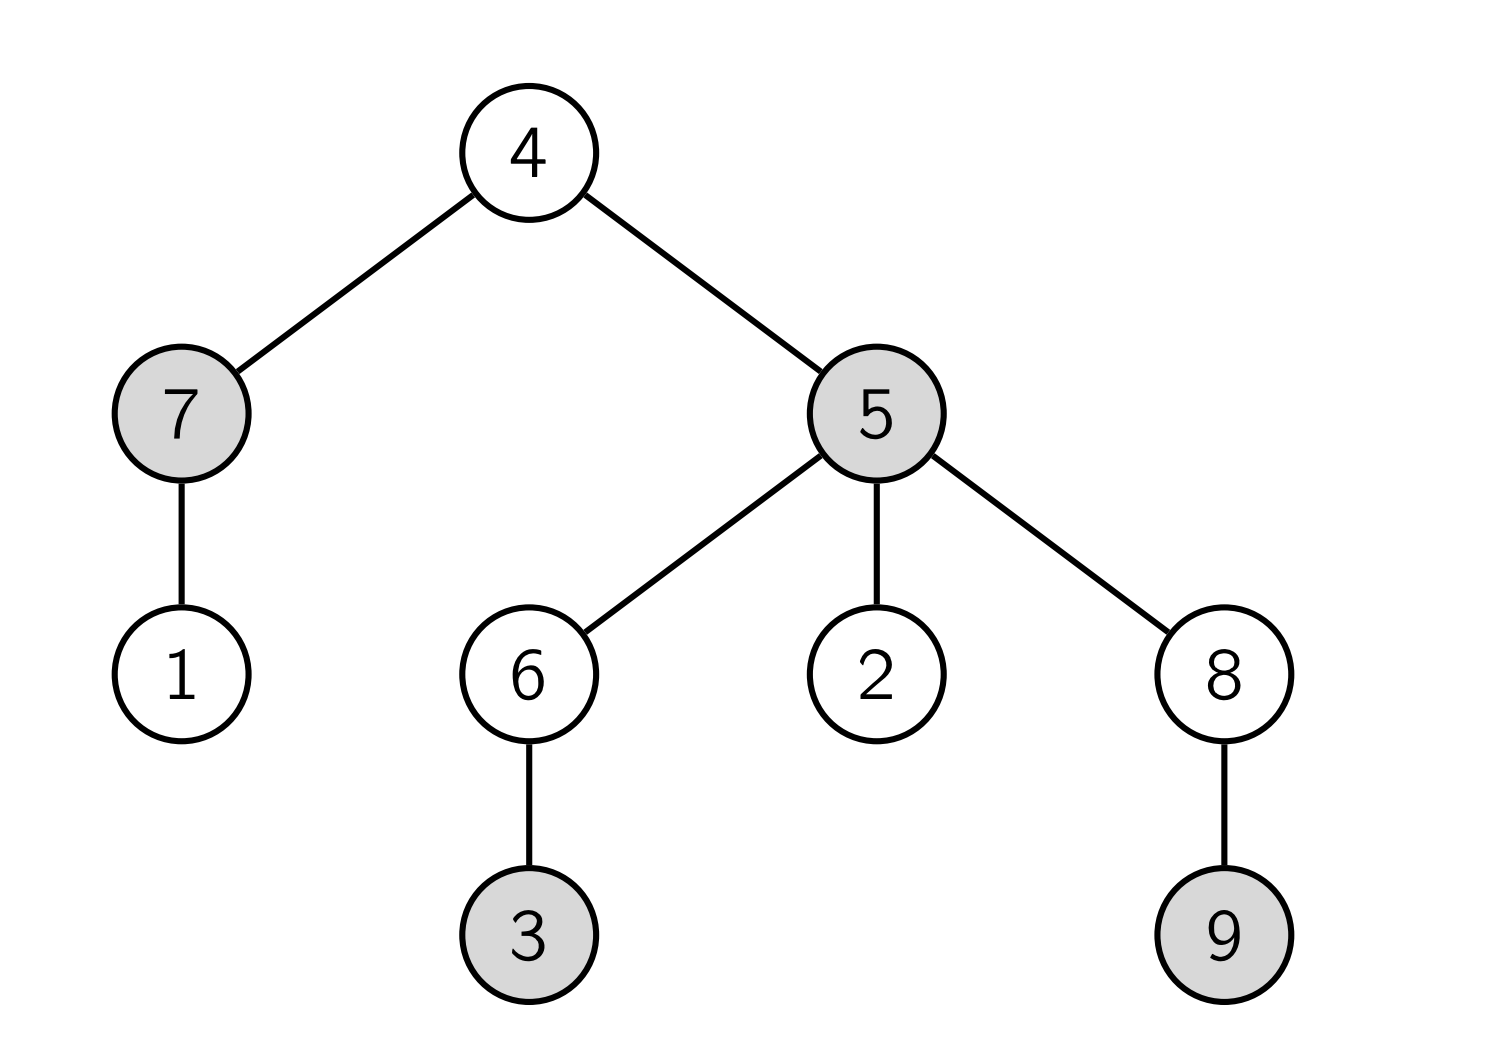
\includegraphics[scale=0.5]{max_is.png}
\end{figure}

As usual, the key question to ask is, ``What should our subproblem(s) be?'' Intuitively, if the problem has to do with trees, then subtrees often play an important role in identifying our subproblems. Let's pick any vertex $r$ and designate it as the root. Denoting the subtree rooted at $u$ as $T_u$, we define $A(u)$ to be the weight of the maximum weight independent set in $T_u$. How can we express $A(u)$ recursively? Letting $S_u$ be the maximum weight independent set of $T_u$, there are two cases:

\begin{enumerate}
    \item If $u \notin S_u$, then $A(u) = \sum_{v} A(v )$ for all children $v$ of $u$.
    \item If $u \in S_u$, then $A(u) = w_u + \sum_{v} A(v )$ for all grandchildren $v$ of $u$. 
\end{enumerate}

To avoid solving the subproblem for trees rooted at grandchildren, we introduce $B(u)$ as the weight of the maximum weight independent set in $T_u \setminus \{u\}$. That is, $B(u) = \sum_{v} A(v )$ for all children $v$ of $u$. Equivalently, we have the following cases: 

\begin{enumerate}
    \item If $u \notin S_u$, then $A(u) = \sum_{v} A(v )$ for all children $v$ of $u$.
    \item If $u \in S_u$, then $A(u) = w_u + \sum_{v} B(v )$ for all children $v$ of $u$. 
\end{enumerate}

So, we can calculate the weight of the maximum weight independent set:
$$
A(u) = \max\left\{w(u) + \sum_{v \in Children(u)} B(u), \sum_{v \in Children(u)} A(v)  \right\}
$$

To create an algorithm out of this recurrence, we can compute the $A(u)$ and $B(u)$ values in a bottom-up manner (a post-order traversal on the tree), arriving at the answer, $A(r)$. This
takes $O(|V|)$ time.




\begin{algorithm}
\caption{MaxWeightIndependentSet(G)}
\label{alg:MaxWeightIndependentSet}
\begin{algorithmic}
\State \texttt{// G is a tree}
\State $r \gets \text{ArbitraryVertex}(G)$
\State $T \gets \text{RootTreeAt}(r)$
\Procedure{SolveSubtreeAt}{$u$}
    \State \eIf{Children$(T, u) = \emptyset$} {
        \State $A(u) \gets w_u$
        \State $B(u) \gets 0$
    }{
        \State \For{$v \in \text{Children}(u)$} {
            \State \texttt{SolveSubTreeAt}(v)
        }
        \State $A(u) \gets \max\left\{\sum_{v \in \text{Children}(u)} A(v), w_u + \sum_{v \in \text{Children}(u)} B(v) \right\}$
        \State $B(u) \gets \sum_{v \in \text{Children}(u)} A(v)$
    }
\EndProcedure
\State \texttt{SolveSubtreeAt}$(r)$
\State \Return $A(r)$
\end{algorithmic}
\end{algorithm}




















\end{document}
